
\newcommand{\FigOverview}{
\begin{figure}[ht]
    \centering
    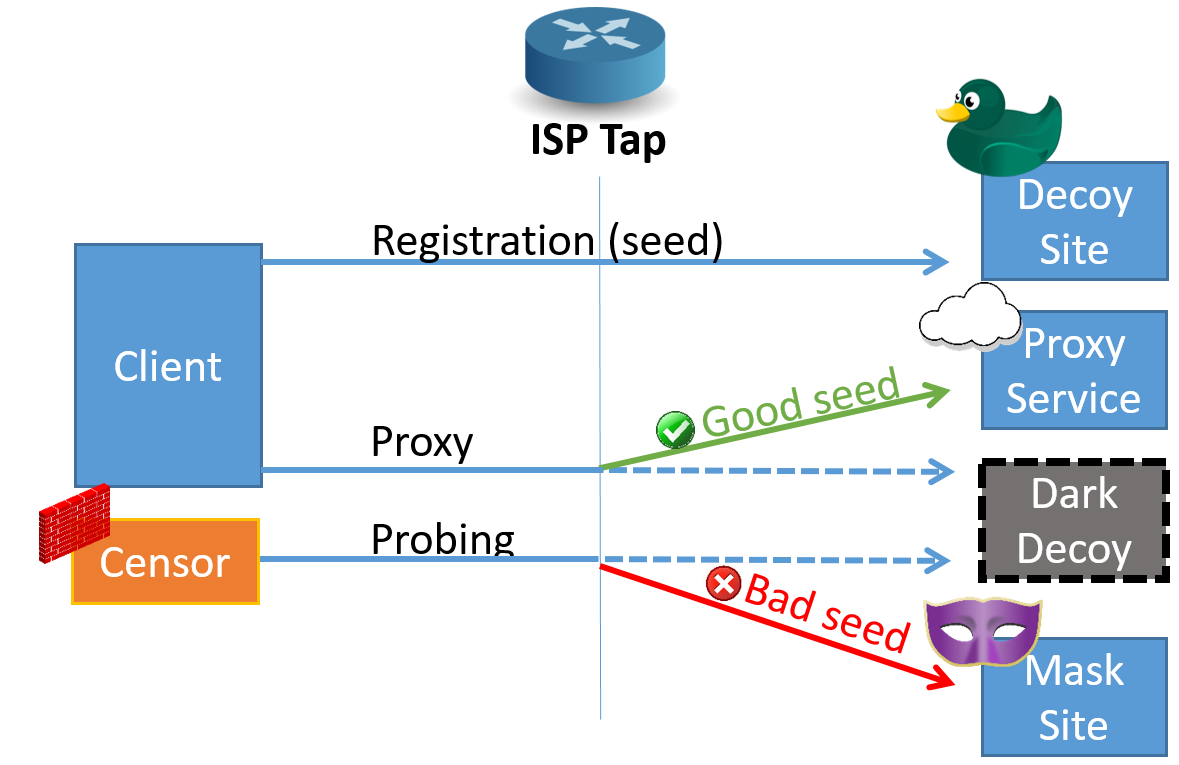
\includegraphics[width=0.9\linewidth,clip]{figures/dark-decoy-overview.png}
    \caption{\textbf{Dark Decoy Overview}\,---\, %
    }
    \label{fig:overview}
\end{figure}
}

\newcommand{\FigHighLevel}{
\begin{figure}[t]
    \centering
    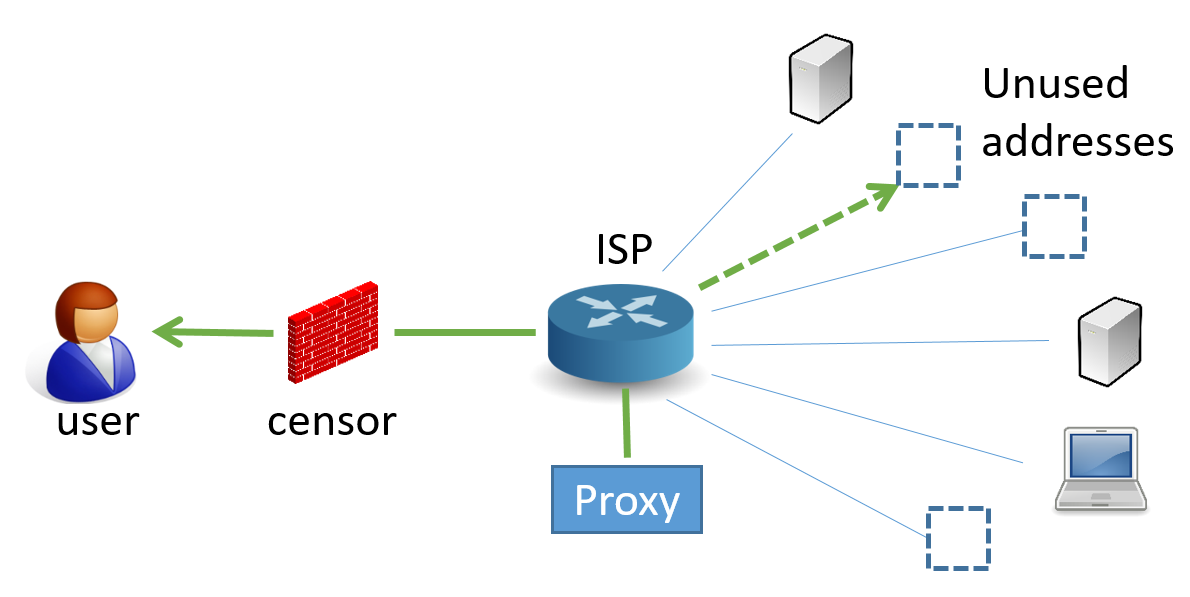
\includegraphics[width=\linewidth,clip]{figures/high-level.png}
    \caption{\textbf{Overview}---%
      When deployed at an ISP, \scheme observes a mirror of inbound and outbound traffic.
      Users request service by embedding a steganographic registration message in a TLS handshake with any reachable site at the ISP\@. Then, the client connects to a random unused (``dark'')
      address in the ISP's AS, and \scheme communicates with the client as if it were that host.
    }
    \label{fig:overview}
\end{figure}
}


\newcommand{\yes}{\CIRCLE}
\newcommand{\no}{\Circle}
\newcommand{\maybe}{\LEFTcircle}

\newcommand{\TabCompare}{
\begin{table*}[ht]
    \centering
    \begin{tabular}{l|cccccccc}
            % Multiflow? Waterfall?
            & \rot{Telex~\cite{telex}} &
            \rot{Cirripede~\cite{cirripede}} &
            \rot{Decoy Routing~\cite{curveball}} &
            \rot{TapDance~\cite{tapdance}} & \rot{Rebound~\cite{rebound}} & \rot{Slitheen~\cite{slitheen}} & \rot{Waterfall~\cite{waterfall}} & \rot{\textbf{Dark Decoys}} \\
            \hline
                                      %Telex Cirr  DR     TD      RB    Slth   Water  DD
            No inline blocking        & \no & \no  & \no & \yes  & \no  & \no  & \no  & \yes \\
            Handles asym. routing     & \no & \yes & \no  & \yes & \yes & \no  & \yes & \yes \\
            Currently deployed        & \no & \no  & \no  & \yes & \no  & \no  & \no  & \no \\
            Replay attack resistant   &\yes & \yes & \yes & \no  & \yes & \yes & \yes & \yes \\
            Traffic analysis resitant &\no  & \no  & \no  & \no  &\maybe& \yes &\maybe& \no \\
            Uses unused addresses     & \no & \no  & \no  & \no  & \no  & \no  & \no  & \yes \\
    \end{tabular}
    %\caption{\textbf{Refraction Networking schemes}\,---\,}
    \label{tab:compare}
\end{table*}
}



\newcommand{\FigImplementation}{
\begin{figure}[ht]
    \centering
    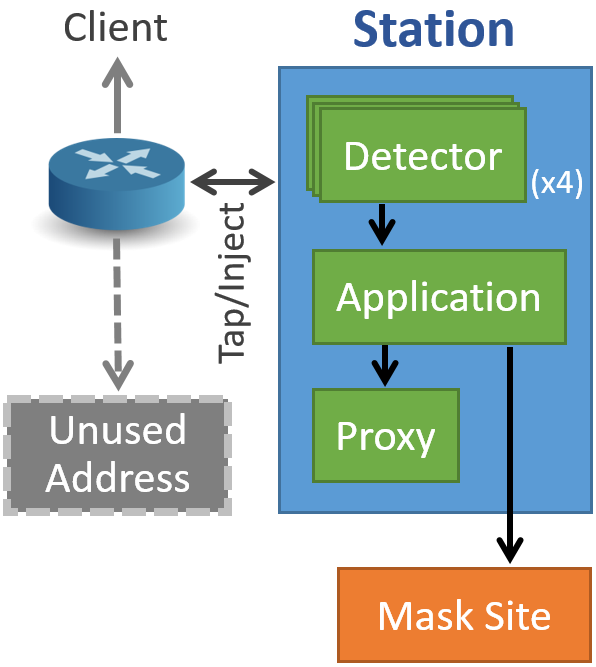
\includegraphics[width=0.7\linewidth,clip]{figures/implementation.png}
    \caption{\textbf{Station Architecture}\,---\, %
    }
    \label{fig:implementation}
\end{figure}
}


